\documentclass[12pt]{article}
\usepackage{times} 			% use Times New Roman font

\usepackage[margin=1in]{geometry}   % sets 1 inch margins on all sides
\usepackage{hyperref}               % for URL formatting
\usepackage[pdftex]{graphicx}       % So includegraphics will work
\setlength{\parskip}{1em}           % skip 1em between paragraphs
\usepackage{indentfirst}            % indent the first line of each paragraph
\usepackage{datetime}
\usepackage[small, bf]{caption}
\usepackage{listings}               % for code listings
\usepackage{xcolor}                 % for styling code
\usepackage{multirow}

%New colors defined below
\definecolor{backcolour}{RGB}{246, 246, 246}   % 0xF6, 0xF6, 0xF6
\definecolor{codegreen}{RGB}{16, 124, 2}       % 0x10, 0x7C, 0x02
\definecolor{codepurple}{RGB}{170, 0, 217}     % 0xAA, 0x00, 0xD9
\definecolor{codered}{RGB}{154, 0, 18}         % 0x9A, 0x00, 0x12

%Code listing style named "gcolabstyle" - matches Google Colab
\lstdefinestyle{gcolabstyle}{
  basicstyle=\ttfamily\small,
  backgroundcolor=\color{backcolour},   
  commentstyle=\itshape\color{codegreen},
  keywordstyle=\color{codepurple},
  stringstyle=\color{codered},
  numberstyle=\ttfamily\footnotesize\color{darkgray}, 
  breakatwhitespace=false,         
  breaklines=true,                 
  captionpos=b,                    
  keepspaces=true,                 
  numbers=left,                    
  numbersep=5pt,                  
  showspaces=false,                
  showstringspaces=false,
  showtabs=false,                  
  tabsize=2
}

\lstset{style=gcolabstyle}      %set gcolabstyle code listing

% to make long URIs break nicely
\makeatletter
\g@addto@macro{\UrlBreaks}{\UrlOrds}
\makeatother

% for fancy page headings
\usepackage{fancyhdr}
\setlength{\headheight}{13.6pt} % to remove fancyhdr warning
\pagestyle{fancy}
\fancyhf{}
\rhead{\small \thepage}
\lhead{\small HW 1, AGUILAR}  % EDIT THIS, REPLACE # with HW number
\chead{\small CS 432, Spring 2021} 
%-------------------------------------------------------------------------
%-------------------------------------------------------------------------
%-------------------------------------------------------------------------
\begin{document}

\begin{centering}
{\large\textbf{HW1-report}}\\ % EDIT THIS
                                % REPLACE # with HW num and ADD title
CARLOS AGUILAR\\                     % EDIT THIS
07 FEBRUARY 2021\\                      % EDIT THIS
\end{centering}

%-------------------------------------------------------------------------

% The * after \section just says to not number the sections
\section*{Q1}
\emph{
Draw the resulting directed graph (either sketch on paper or use another tool) showing how the nodes are connected to each other and include an image in your report. This does not need to fit into the bow-tie type diagram, but should look more similar to the graph on slide 24 from Module-01 Web-Science-Architecture.}

\subsection*{Answer}
The nodes from the graph are listed in alphabetical order in each of the following categories:
Figure \ref{fig:qb1} shows the bowtie graph drawn with jflap.

\begin{figure}[h!]
    \centering
    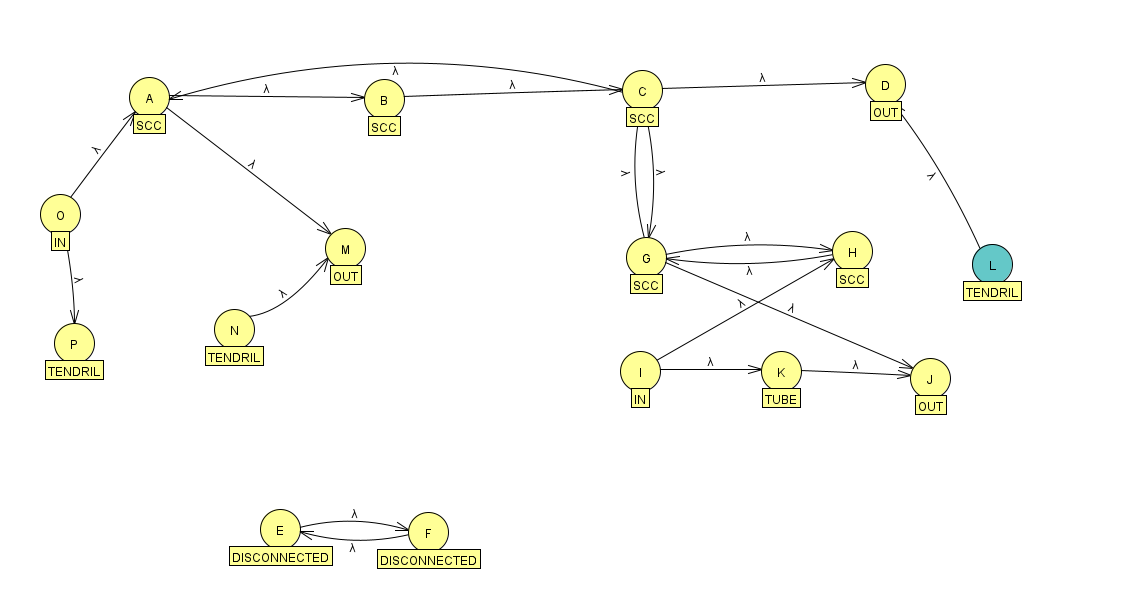
\includegraphics[clip, width=\textwidth] {bowtie}
    \caption{Web Browser User-Agent HTTP Header}
    \label{fig:bowtie}
\end{figure}

\begin{itemize}
  \item SCC: A, B, C, G, H
  \item IN: I, O
  \item OUT: D, J, M
  \item Tendrils: L(IN Reachable), N(IN Reachable), P(OUT Reachable)
  \item Tubes: K (Allows I to go through it to get to J)
  \item Disconnected: E, F
\end{itemize}

\subsection*{Discussion}
The most apparent nodes were the disconnected E and F, then came the Tube, which I believe K was the only tube present. Although B provided only a passage from A to C, I believed A and C were still SCC. Therefore B must always be SCC. The tendrils L, N, and P were slightly challenging to decide on, but since they only had a single point of entry or exit followed by not further transitions, I concluded that they must be tendrils.  I decided on the In and Out by thinking of how many entrances or exits a single node holds. If it had all in and more than one, then it was an IN. Conversely, if it contained more OUTs, then it was an OUT.
%-  *******  Fill this out *******

%-------------------------------------------------------------------------
%-------------------------------------------------------------------------
\section*{Q2}
\emph{Demonstrate that you know how to use curl and are familiar with the available options.}

%URI to request: \url{http://www.cs.odu.edu/~mweigle/courses/cs532/ua_echo.php}

\subsection*{Answer}
a) Figure \ref{fig:q2a} is a screenshot of my browser and the resulting webpage showing the User-Agent HTTP header that the web browser sends to the web server.

\begin{figure}[h!]
    \centering
    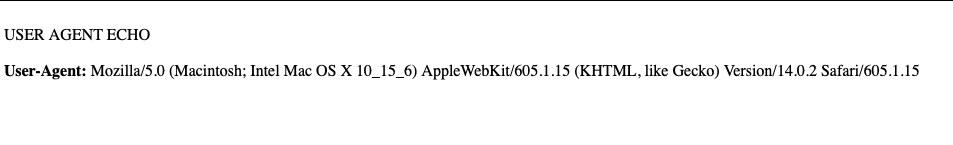
\includegraphics[clip, width=\textwidth] {a}
    \caption{Web Browser User-Agent HTTP Header}
    \label{fig:q2a}
\end{figure}

b) Figure \ref{fig:qb1} shows the single curl command, requesting the URI, showing the HTTP response headers, following any redirects, and changes the User-Agent HTTP request field to "CS432/532". 

\begin{figure}[h!]
    \centering
    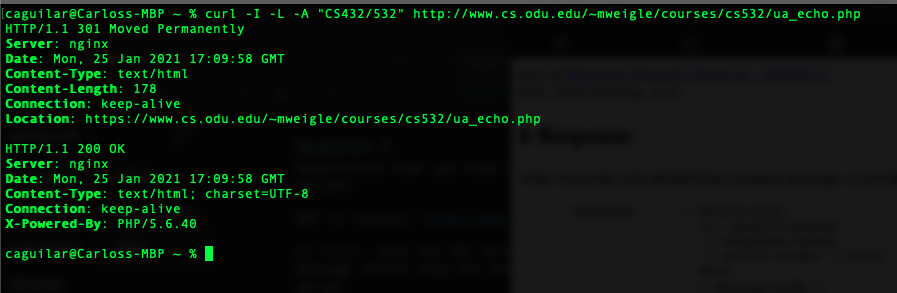
\includegraphics[clip, width=\textwidth] {b1}
    \caption{Question 2 b - 1}
    \label{fig:qb1}
\end{figure}

Figure \ref{fig:qb2} shows the result of my execution on the command line.

\begin{figure}[h!]
    \centering
    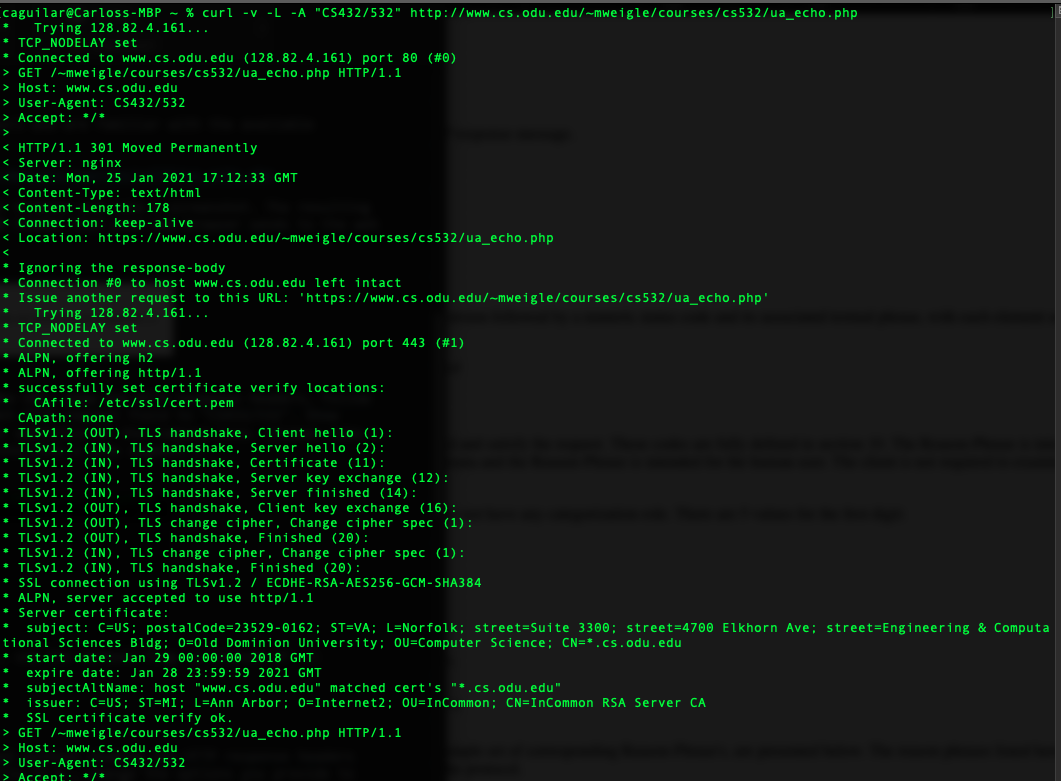
\includegraphics[clip, width=\textwidth] {b2}
    \caption{Question 2 b - 2}
    \label{fig:qb2}
\end{figure}


c) Figure \ref{fig:qc1} shows the same command used, but without showing the HTTP response headers and with saving the HTML output to a file.

\begin{figure}[h!]
    \centering
    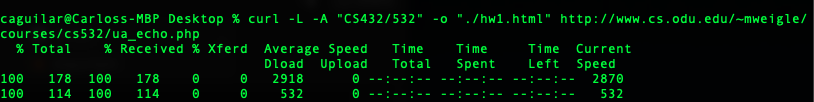
\includegraphics[clip, width=\textwidth] {c1}
    \caption{Question 2 c - 1}
    \label{fig:qc1}
\end{figure}


Figure \ref{fig:qc2} shows the HTML output file that was produced by curl in a web browser.

\begin{figure}[h!]
    \centering
    % trim and clip are used to crop the image, trim=left bottom right top
    % width sets max width, height will be scaled appropriately
    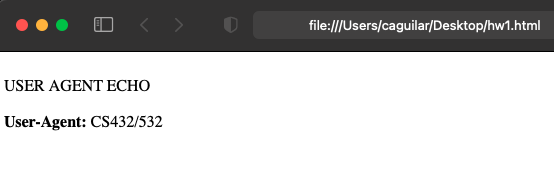
\includegraphics[clip, width=\textwidth] {c2}
    \caption{Question 2 c - 2}
    \label{fig:qc2}
\end{figure}

\subsection*{Discussion}
With the curl command, I could use manipulate the User-Agent and save the content to file: hw1.html then view it on the web browser. The screenshots above illustrate how I could view the headers and manipulate the webpage then save it to an output file.

%-  *******  Fill this out *******

%-------------------------------------------------------------------------
%-------------------------------------------------------------------------

\section*{Q3}
\emph{
Write a Python program to find links to PDFs in a webpage.
Your program must do the following:
\begin{itemize}
    \item Take the URI of a webpage as a command-line argument
    \item Extract all the links from the page
    \item For each link, request the URI and use the Content-Type HTTP response header to determine if the link references a PDF file
    \item For all links that reference a PDF file, print the original URI (found in the source of the original HTML), the final URI (after any redirects), and the number of bytes in the PDF file. (Hint: Content-Length HTTP response header)
\end{itemize}
}
\subsection*{Answer}
Listing \ref{lst:import} fulfills all the requirements listed above and can be executed with any given URI.

%Importing code from file
\lstinputlisting[language=Python, caption=Python code for finding pdfs, label=lst:import]{cs432-hw1.py}

\subsection*{Discussion}

The python program works for searching through any given URI. If the provided URI does not have any pdf files, it will not output any results.  The complexity is a little too high, and I need to work on that. Additionally, I need to work on adding formatting to outputs.

\begin{figure}[h!]
    \centering
    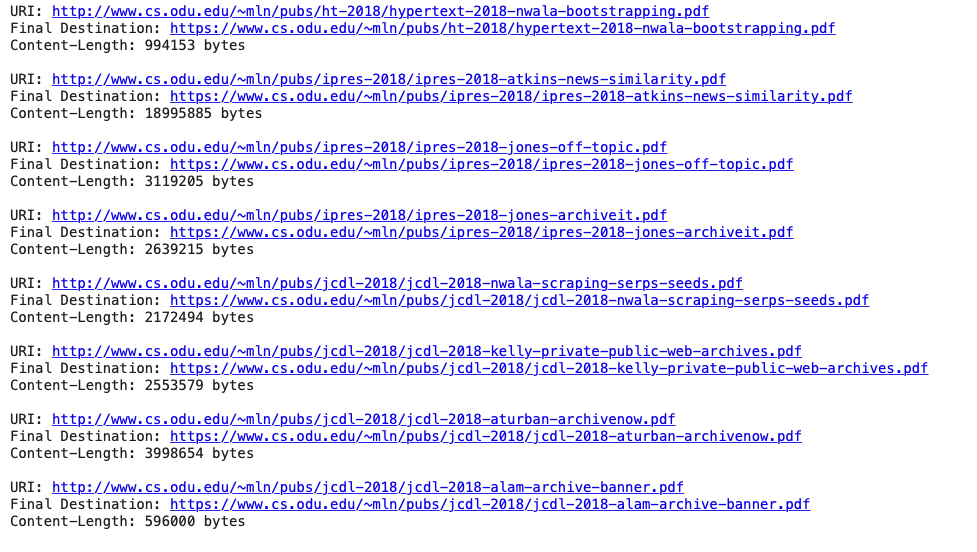
\includegraphics[clip, width=\textwidth] {pdf-1}
    \caption{List of PDF and output}
    \label{fig:p1}
\end{figure}

%-  *******  Add more *******
%-------------------------------------------------------------------------

\end{document}

